\section{Material und Methoden} % (fold)
    \label{sec:material_und_methoden}
    Es werden drei Versuchsmedien erstellt, um das Wachstum differenziert betrachten zu können. Dabei wird eines mit normalem Leitungswasser gewässert, eines mit Salzwasser und eines mit angesäuertem Wasser. Der Salzgehalt von Zweitem soll bei $0,1 \frac{mol}{l}$ liegen. Dementsprechend werden dazu 5,85g NaCl in 100ml Leitungswasser gelöst und anschließend zu einem Liter aufgefüllt (Werte siehe \autoref{equ:nacl}).
    \begin{equation}\label{equ:nacl}
        \begin{split}  
        m(NaCl) &= 0,1\frac{mol}{l} * V(H_2O) * M(NaCl)\\
        &= 0,1\frac{mol}{l} * 1l * 58,5\frac{g}{mol}\\
        & = 5,85g
        \end{split}
    \end{equation}
    Das saure Medium soll einen pH-Wert von 5 haben. Zur Verfügung steht Essigessenz mit dem pH-Wert 2,65, sodass von dieser 4,5ml zu einem Liter aufgefüllt werden (siehe \autoref{equ:essig}).
    \begin{equation}
        \label{equ:essig}
        \begin{split}
            pH(Essig) & = 2,65 \\
            \Rightarrow c(H^+)_{alt} &=10^{-2,65}\\
            c(H^+)_{neu}&=10^{-5}\ \ \ \ =10^{-2,65} * x\\
            x&=\frac{10^{-5}}{10^{-2,65}} =0,0045
        \end{split}
    \end{equation}
    In folgender \autoref{tab:materials} sind alle verwendeten Materialien aufgelistet, samt Menge, Art der Verwendung und zusätzlichen relevanten Informationen.
    \begin{table}[h]
        \caption{Materialien}
        \label{tab:materials}
        \csvreader[tabular=rrrr,
            respect percent,
            table head=\toprule\centerIt{\textbf{Material}} & \centerIt{\textbf{Menge}} & \centerIt{\textbf{Zweck}} & \centerIt{\textbf{Zusatzinfo}}\\\midrule,
            /csv/separator=semicolon,
            head to column names,
            late after last line=\\\bottomrule]
            {../Materials.csv}{}
            {\Material&\Menge&\Zweck&\Zusatzinfo}
    \end{table}

    \newpage
    \subsection{Durchführung} % (fold)
        \label{sub:durchführung}
        An Tag 0 wird das Experiment vorbereitet. Dazu werden die drei Tassen jeweils bis zum Rand mit Watte gefüllt, so dass eine ebene Oberfläche entsteht. Darauf werden nun mithilfe einer Pinzette die Samen rasterförmig positioniert, also je Tasse 5 Reihen mit je 4 Samen (siehe \autoref{fig:exp_prep}). Die Tassen werden nun in einer Reihe aufgestellt, nicht direkt am Fenster, sondern in der Mitte des Raumes, sodass sie den ganzen Tag über Tageslicht haben, aber nicht direkt in der prallen Sonne oder im Durchzug des Fensters stehen.

        Die Vorbereitung der Nährmedien erfolgt der Reihe nach. Zuerst wird das Glas für das neutrale Medium mit Leitungswasser (LW) ausgespült und dann erneut voll aufgefüllt.

        Dann wird der Messbecher ausgespült und das Salz in das entsprechende Glas gegeben. Diesem Glas werden 100 ml LW zugegeben, in welchem das Salz schwenkend gelöst wird. Die Lösung wird nun in den Messbecher gegeben, dann das Glas mit deutlich weniger als einem Liter LW aufgefüllt, geschwenkt und auch in den Becher gegeben, um Restlösung mit zu übertragen. Im Anschluss wird der Messbecher mit LW zu einem Liter aufgefüllt. Die fertige 0,1-molare NaCl-Lösung wird nun in das eben geleerte Glas gegeben.

        Für die Herstellung des sauren Mediums wird der Messbecher zwei mal gründlich ausgespült und diesem dann darauffolgend das abgemessene Essig zugegeben. Dieses befand sich in einem separaten 156 ml Gefäß, welches vor der Nutzung auch gereinigt wurde und nun mit LW halb aufgefüllt, geschwenkt, und auch in den Messbecher geleert wird, um Restflüssigkeit mitzunehmen. Der Messbecher wird nun geschwenkt, zu einem Liter aufgefüllt und dessen Inhalt folglich in das dritte Gefäß für das saure Medium gefüllt.

        Die eindeutig voneinander unterscheidbaren Gläser mit entsprechenden Medien werden hinter ihre zugehörigen Tassen gestellt (siehe \autoref{fig:exp_prep}).
        \begin{figure}[h]
            \centering
            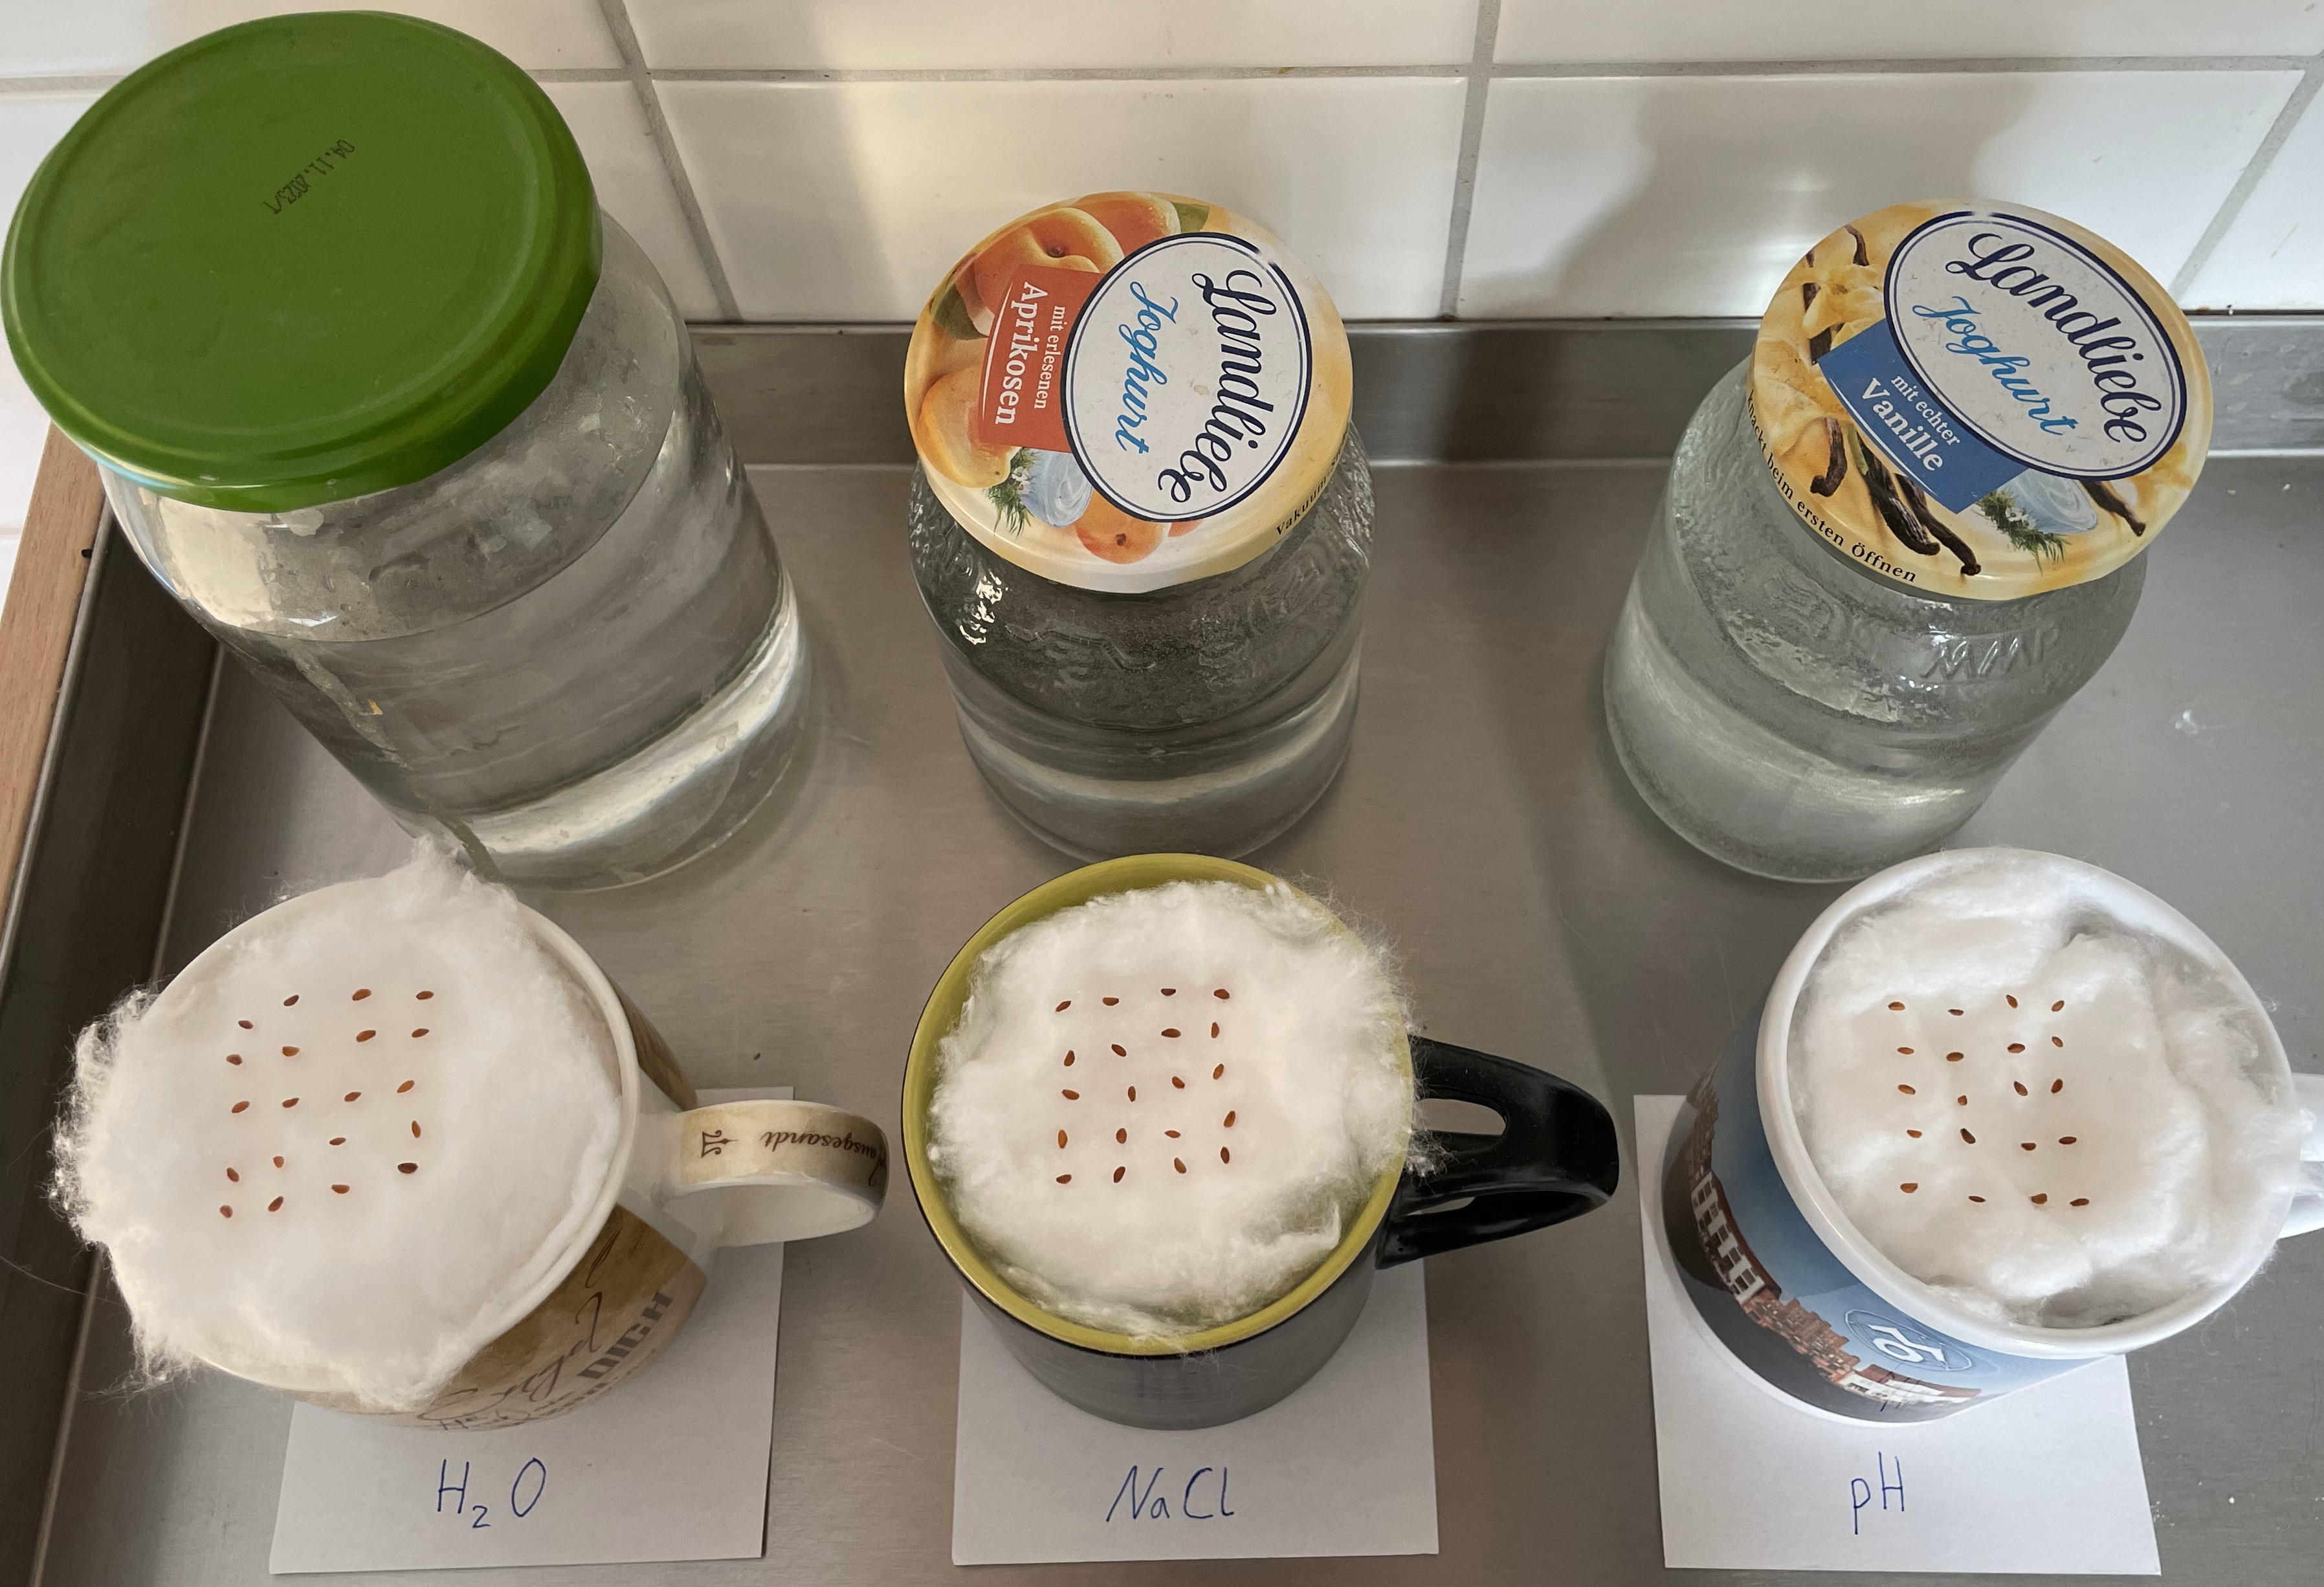
\includegraphics[width=.7\textwidth]{preparation.png}
            \caption{Vorbereitung des Experiments}
            \label{fig:exp_prep}
        \end{figure}

        \newpage
        An jedem Messtag, einschließlich Tag 0, werden dieselben Schritte in derselben Reihenfolge durchgeführt.
        \begin{enumerate}[1.]
            \item Messen und notieren der Wuchshöhen jedes einzelnen Samens der neutralen Probe mit dem Maßband
            \item gleichmäßiges Gießen des Samenrasters mit drei Teelöffeln aus dem neutralen Medium
            \item anschließendes Wiederholen der vorigen Schritte für die salzige und zum Schluss der sauren Probe
        \end{enumerate}
        Tagsüber wird das Zimmer nicht künstlich verdunkelt, das Fenster ist durchgängig angekippt. Beim Messen selbst wird künstliches weißes Licht verwendet, um die Stängel besser unterscheiden zu können. Zudem werden die Blätter mit in die Wuchshöhe mit einbezogen.

        Mit dem ersten Gießen startet die Erfassung der Wuchshöhen, alle somit zuerst\\bei 0 mm.
    
    % subsection durchführung (end)
% section material_und_methoden (end)
